\subsection{Over-/Underfitting and Cross Validation}
    \begin{itemize}
        \item Underfitting: model is too simplistic to capture the underlying patterns in the data
        \item Overfitting: model memorizes random fluctuations in the data rather than capturing the underlying patterns
    \end{itemize}
    Result: No liable predictions from the model\\
    Solution: Cross-Validation
    \begin{enumerate}
        \item subdivide data set into smaller parts
        \item use n-1 parts for training and 1 remaining part for testing, trying out different settings
    \end{enumerate}
    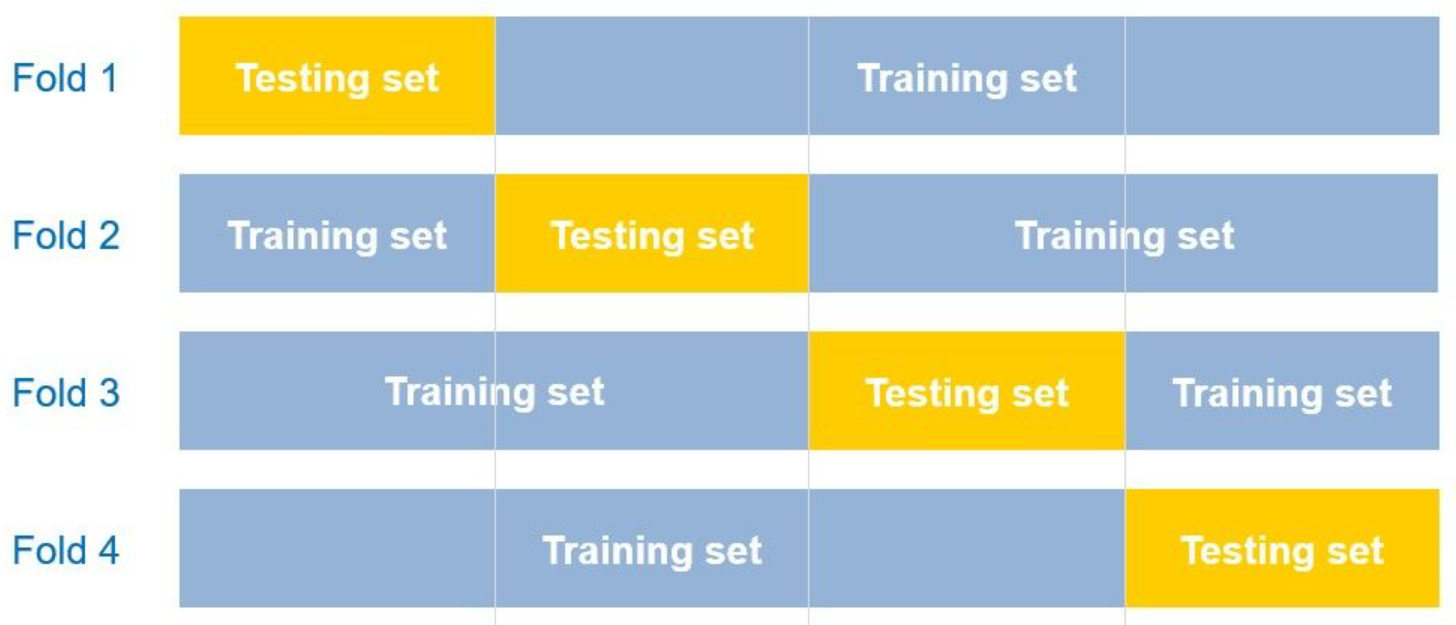
\includegraphics[width = \linewidth]{src/8_ml/images/cross_validation.png}